% Options for packages loaded elsewhere
\PassOptionsToPackage{unicode}{hyperref}
\PassOptionsToPackage{hyphens}{url}
\PassOptionsToPackage{dvipsnames,svgnames,x11names}{xcolor}
%
\documentclass[
  letterpaper,
  DIV=11,
  numbers=noendperiod]{scrartcl}

\usepackage{amsmath,amssymb}
\usepackage{iftex}
\ifPDFTeX
  \usepackage[T1]{fontenc}
  \usepackage[utf8]{inputenc}
  \usepackage{textcomp} % provide euro and other symbols
\else % if luatex or xetex
  \usepackage{unicode-math}
  \defaultfontfeatures{Scale=MatchLowercase}
  \defaultfontfeatures[\rmfamily]{Ligatures=TeX,Scale=1}
\fi
\usepackage{lmodern}
\ifPDFTeX\else  
    % xetex/luatex font selection
\fi
% Use upquote if available, for straight quotes in verbatim environments
\IfFileExists{upquote.sty}{\usepackage{upquote}}{}
\IfFileExists{microtype.sty}{% use microtype if available
  \usepackage[]{microtype}
  \UseMicrotypeSet[protrusion]{basicmath} % disable protrusion for tt fonts
}{}
\makeatletter
\@ifundefined{KOMAClassName}{% if non-KOMA class
  \IfFileExists{parskip.sty}{%
    \usepackage{parskip}
  }{% else
    \setlength{\parindent}{0pt}
    \setlength{\parskip}{6pt plus 2pt minus 1pt}}
}{% if KOMA class
  \KOMAoptions{parskip=half}}
\makeatother
\usepackage{xcolor}
\usepackage{svg}
\setlength{\emergencystretch}{3em} % prevent overfull lines
\setcounter{secnumdepth}{-\maxdimen} % remove section numbering
% Make \paragraph and \subparagraph free-standing
\makeatletter
\ifx\paragraph\undefined\else
  \let\oldparagraph\paragraph
  \renewcommand{\paragraph}{
    \@ifstar
      \xxxParagraphStar
      \xxxParagraphNoStar
  }
  \newcommand{\xxxParagraphStar}[1]{\oldparagraph*{#1}\mbox{}}
  \newcommand{\xxxParagraphNoStar}[1]{\oldparagraph{#1}\mbox{}}
\fi
\ifx\subparagraph\undefined\else
  \let\oldsubparagraph\subparagraph
  \renewcommand{\subparagraph}{
    \@ifstar
      \xxxSubParagraphStar
      \xxxSubParagraphNoStar
  }
  \newcommand{\xxxSubParagraphStar}[1]{\oldsubparagraph*{#1}\mbox{}}
  \newcommand{\xxxSubParagraphNoStar}[1]{\oldsubparagraph{#1}\mbox{}}
\fi
\makeatother


\providecommand{\tightlist}{%
  \setlength{\itemsep}{0pt}\setlength{\parskip}{0pt}}\usepackage{longtable,booktabs,array}
\usepackage{calc} % for calculating minipage widths
% Correct order of tables after \paragraph or \subparagraph
\usepackage{etoolbox}
\makeatletter
\patchcmd\longtable{\par}{\if@noskipsec\mbox{}\fi\par}{}{}
\makeatother
% Allow footnotes in longtable head/foot
\IfFileExists{footnotehyper.sty}{\usepackage{footnotehyper}}{\usepackage{footnote}}
\makesavenoteenv{longtable}
\usepackage{graphicx}
\makeatletter
\newsavebox\pandoc@box
\newcommand*\pandocbounded[1]{% scales image to fit in text height/width
  \sbox\pandoc@box{#1}%
  \Gscale@div\@tempa{\textheight}{\dimexpr\ht\pandoc@box+\dp\pandoc@box\relax}%
  \Gscale@div\@tempb{\linewidth}{\wd\pandoc@box}%
  \ifdim\@tempb\p@<\@tempa\p@\let\@tempa\@tempb\fi% select the smaller of both
  \ifdim\@tempa\p@<\p@\scalebox{\@tempa}{\usebox\pandoc@box}%
  \else\usebox{\pandoc@box}%
  \fi%
}
% Set default figure placement to htbp
\def\fps@figure{htbp}
\makeatother

\KOMAoption{captions}{tableheading}
\makeatletter
\@ifpackageloaded{caption}{}{\usepackage{caption}}
\AtBeginDocument{%
\ifdefined\contentsname
  \renewcommand*\contentsname{Table of contents}
\else
  \newcommand\contentsname{Table of contents}
\fi
\ifdefined\listfigurename
  \renewcommand*\listfigurename{List of Figures}
\else
  \newcommand\listfigurename{List of Figures}
\fi
\ifdefined\listtablename
  \renewcommand*\listtablename{List of Tables}
\else
  \newcommand\listtablename{List of Tables}
\fi
\ifdefined\figurename
  \renewcommand*\figurename{Figure}
\else
  \newcommand\figurename{Figure}
\fi
\ifdefined\tablename
  \renewcommand*\tablename{Table}
\else
  \newcommand\tablename{Table}
\fi
}
\@ifpackageloaded{float}{}{\usepackage{float}}
\floatstyle{ruled}
\@ifundefined{c@chapter}{\newfloat{codelisting}{h}{lop}}{\newfloat{codelisting}{h}{lop}[chapter]}
\floatname{codelisting}{Listing}
\newcommand*\listoflistings{\listof{codelisting}{List of Listings}}
\makeatother
\makeatletter
\makeatother
\makeatletter
\@ifpackageloaded{caption}{}{\usepackage{caption}}
\@ifpackageloaded{subcaption}{}{\usepackage{subcaption}}
\makeatother

\usepackage{bookmark}

\IfFileExists{xurl.sty}{\usepackage{xurl}}{} % add URL line breaks if available
\urlstyle{same} % disable monospaced font for URLs
\hypersetup{
  pdftitle={MATLAB Behavioural Documentation},
  colorlinks=true,
  linkcolor={blue},
  filecolor={Maroon},
  citecolor={Blue},
  urlcolor={Blue},
  pdfcreator={LaTeX via pandoc}}


\title{MATLAB Behavioural Documentation}
\author{}
\date{}

\begin{document}
\maketitle


\begin{figure}[H]

{\centering \pandocbounded{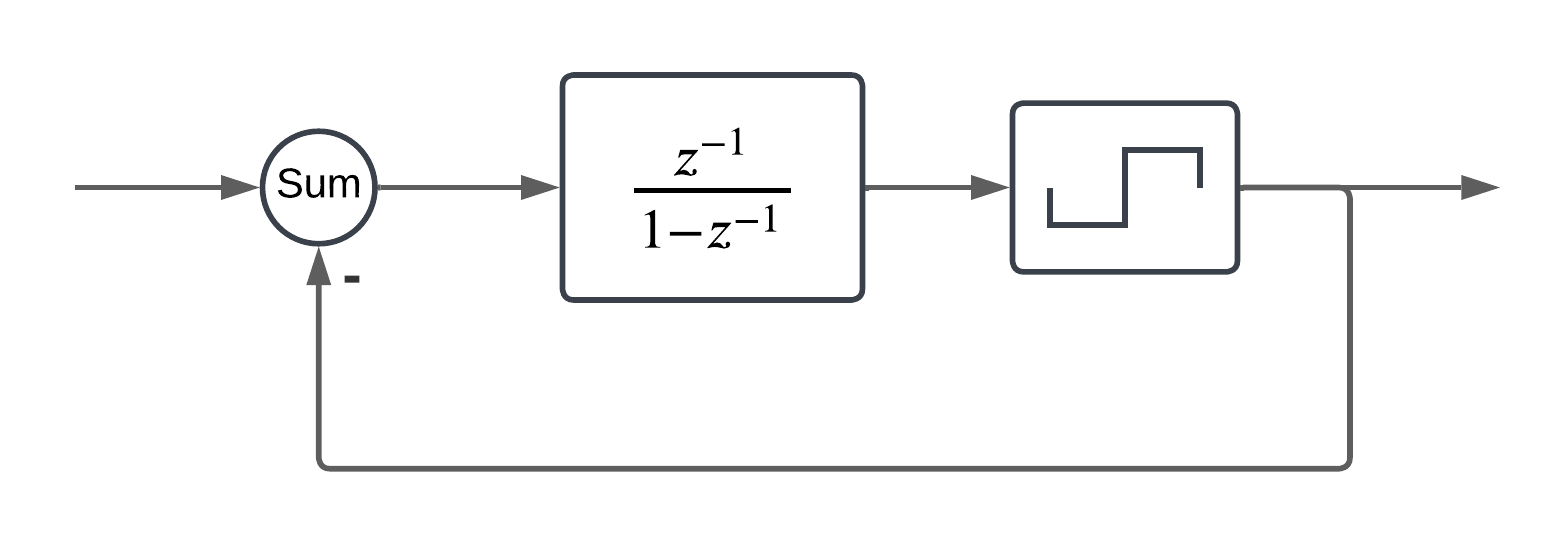
\includegraphics[keepaspectratio]{../recources/pictures/1st_Order_MOD_behav.png}}

}

\caption{Blockdiagram of 1st order modulator}

\end{figure}%

\subsection{1st Order Modulator Model:}\label{st-order-modulator-model}

\subsubsection{Comprised of:}\label{comprised-of}

\begin{itemize}
\tightlist
\item
  sum block (\(\Delta\)):

  \begin{itemize}
  \tightlist
  \item
    one positive and one negativ input
  \item
  \end{itemize}
\item
  discrete-time integrator as accumulator:

  \begin{itemize}
  \tightlist
  \item
    realised as: \(\frac{z^{-1}}{1-z^{-1}}\)
  \item
  \end{itemize}
\item
  comparator (non-linear element):

  \begin{itemize}
  \tightlist
  \item
    switching threshold defined with `eps' := \(2^{-52}\) = 2.2204e-16

    \begin{itemize}
    \tightlist
    \item
      essentially switches around `0'-crossovers\\
    \end{itemize}
  \item
    output either `1' (on) or `-1' (off)
  \end{itemize}
\item
  feedback path from comparator output to sum block (neg. sign)
\end{itemize}

\begin{figure}[H]

{\centering \pandocbounded{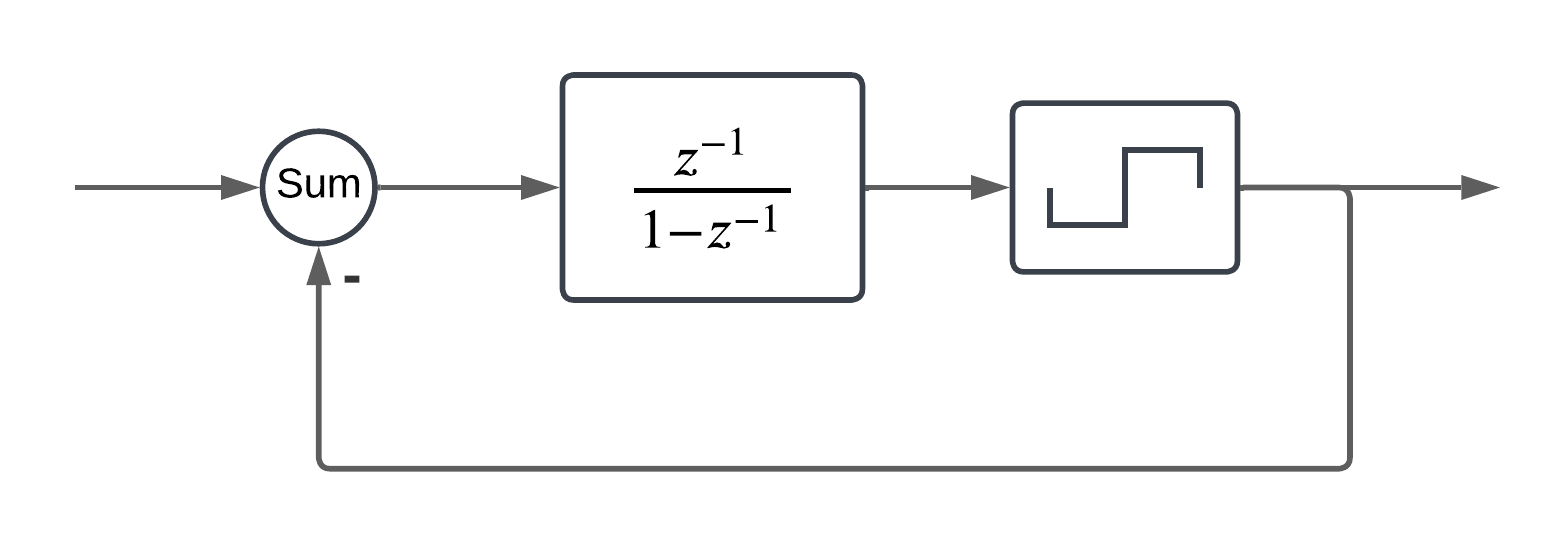
\includegraphics[keepaspectratio]{../recources/pictures/1st_Order_MOD_behav.png}}

}

\caption{Behavioural Model of 1st Order Modulator}

\end{figure}%

\subsubsection{In-Depth description:}\label{in-depth-description}

\subparagraph{Input signal:}\label{input-signal}

\begin{itemize}
\tightlist
\item
  Analog signal

  \begin{itemize}
  \tightlist
  \item
    Conveniently a sinusoid

    \begin{itemize}
    \tightlist
    \item
      Is non-linear, yet periodicly predictable
    \end{itemize}
  \end{itemize}
\end{itemize}

\subparagraph{\texorpdfstring{Delta
(\(\Delta\)):}{Delta (\textbackslash Delta):}}\label{delta-delta}

\begin{itemize}
\tightlist
\item
  Feedback-node of the system
\end{itemize}

\subparagraph{\texorpdfstring{Integrator/ Loop Filter
(\(\Sigma\))}{Integrator/ Loop Filter (\textbackslash Sigma)}}\label{integrator-loop-filter-sigma}

\begin{itemize}
\tightlist
\item
  Discrete-time implementation of integrator =\textgreater{} accumulator

  \begin{itemize}
  \tightlist
  \item
    also represents a lowpass filter
  \item
    Includes a delay of one time step.
  \end{itemize}
\item
  Serves as the ``loop filter'' of our system.

  \begin{itemize}
  \tightlist
  \item
    Accumulates difference (``error'') between input and quantized
    feedback, including a sample delay.
  \item
    Modeled, using the expression: \[
    \frac{z^{-1}}{1-z^{-1}}
    \]
  \end{itemize}
\item
  System relevance:

  \begin{enumerate}
  \def\labelenumi{\arabic{enumi}.}
  \tightlist
  \item
    Accumulation of input signal
  \item
    Shaping of Quantization Noise (\(\textit{Noise Shaping}\))
  \end{enumerate}
\end{itemize}

\subsection{2nd Order Modulator Model:}\label{nd-order-modulator-model}

\subsubsection{Comprised of
(additional):}\label{comprised-of-additional}

\begin{itemize}
\tightlist
\item
  sum block (\(\delta\)):

  \begin{itemize}
  \tightlist
  \item
    one positive and one negativ input
  \end{itemize}
\item
  discrete integrator/ loopfilter:

  \begin{itemize}
  \tightlist
  \item
    realised as: \(\frac{z^{-1}}{1-z^{-1}}\)
  \end{itemize}
\item
  coefficient driven gains after integrators and before \(\delta\)s
\end{itemize}

\begin{figure}[H]

{\centering \pandocbounded{\includesvg[keepaspectratio]{../recources/pictures/Mod_2nd_Order.svg}}

}

\caption{Blockdiagram of 2nd Order Modulator}

\end{figure}%




\end{document}
